\documentclass[12pt,a4paper]{paper}
\usepackage[utf8]{inputenc}
\usepackage[english]{babel}
\usepackage{amsmath}
\usepackage{enumitem}
\usepackage{amsfonts}
\usepackage{amssymb}
\usepackage[left=2cm,right=2cm,top=2cm,bottom=2cm]{geometry}
\usepackage{Sweave}
\begin{document}
\title{STAT646 - Homework 2\\\small{Daniel Osorio - dcosorioh@tamu.edu\\Department of Veterinary Integrative Biosciences\\Texas A\&M University}}
\maketitle
\Sconcordance{concordance:Osorio_Daniel_HW2.tex:Osorio_Daniel_HW2.Rnw:%
1 8 1 1 0 5 1 1 2 1 0 1 3 2 0 2 1 1 3 2 0 5 1 3 0 1 2 2 1 1 2 1 0 3 1 3 %
0 1 2 1 1 1 2 6 0 1 1 5 0 1 1 6 0 1 2 1 1 1 2 1 0 1 2 1 0 1 1 1 2 1 0 1 %
1 1 2 1 0 1 1 4 0 1 2 2 1 1 2 1 0 2 1 1 11 10 0 4 1 4 0 1 2 7 1 1 4 3 0 %
1 1 3 0 1 2 1 1 1 2 1 0 3 1 4 0 1 2 1 1 1 2 1 0 2 1 4 0 1 2 1 1 1 2 1 0 %
1 1 4 0 1 2 4 1 1 2 1 0 5 1 15 0 1 14 2 1}

\begin{enumerate}
\item For the yeast data, do the following:
\begin{Schunk}
\begin{Sinput}
> yeastFiles <- list.files("yeastData/", full.names = TRUE)
> yeastInfo <- lapply(yeastFiles, function(file){
+   read.csv(file, sep = "\t", comment.char = "!")
+ })
> spots <- table(unlist(lapply(yeastInfo, function(X){X[,1]})))
> spots <- names(spots)[spots == length(yeastInfo)]
> yeastInfo <- lapply(yeastInfo, function(X){
+     X[X[,1] %in% spots,c("Ch1.Intensity..Median.","Ch2.Intensity..Median.")]
+ })
> sNames <- gsub(".txt$","",basename(yeastFiles))
> sNames <- gsub("[[:alpha:]]","",sNames)
> chanel1 <- sapply(yeastInfo, function(X){X[,1]})
> chanel2 <- sapply(yeastInfo, function(X){X[,2]})
> colnames(chanel1) <- colnames(chanel2) <- sNames
> rownames(chanel1) <- rownames(chanel2) <- spots
> Y <- log2(chanel2) - log2(chanel1)
\end{Sinput}
\end{Schunk}
\begin{enumerate}
\item For each of average, complete, and single linkage, carry out hierarchical clustering on
the samples using Euclidean distance.
\begin{Schunk}
\begin{Sinput}
> distanceMatrix <- dist(t(Y))
> avgHclust <- hclust(distanceMatrix, method = "average")
> sglHclust <- hclust(distanceMatrix, method = "single")
> cptHclust <- hclust(distanceMatrix, method = "complete")
\end{Sinput}
\end{Schunk}
\begin{enumerate}
\item Which two samples are merged first, and what is the distance between them?
\begin{Schunk}
\begin{Sinput}
> c(sNames[abs(avgHclust$merge[1,])], round(avgHclust$height[1],2))
\end{Sinput}
\begin{Soutput}
[1] "69976" "69977" "17.37"
\end{Soutput}
\begin{Sinput}
> c(sNames[abs(sglHclust$merge[1,])], round(sglHclust$height[1],2))
\end{Sinput}
\begin{Soutput}
[1] "69976" "69977" "17.37"
\end{Soutput}
\begin{Sinput}
> c(sNames[abs(cptHclust$merge[1,])], round(cptHclust$height[1],2))
\end{Sinput}
\begin{Soutput}
[1] "69976" "69977" "17.37"
\end{Soutput}
\end{Schunk}
\item Report a height plot showing merge distances. How many clusters would you say
there are? \textit{Depending of the linkage method, between 2 and 4.}
\begin{Schunk}
\begin{Sinput}
> par(mfrow=c(2,3), mar=c(3,3,1,1))
> plot(avgHclust$height)
> abline(h = 60.5, col = "red", lty = 2)
> plot(sglHclust$height)
> abline(h = 44.5, col = "red", lty = 2)
> plot(cptHclust$height)
> abline(h = 71.35, col = "red", lty = 2)
> par(mar=c(3,2,1,4))
> plot(as.dendrogram(avgHclust), horiz = TRUE, 
+      main = "Average Linkage")
> abline(v = 60.5, lty = 2, col= "red")
> plot(as.dendrogram(sglHclust), horiz = TRUE, 
+      main = "Single Linkage")
> abline(v = 44.5, lty = 2, col= "red")
> plot(as.dendrogram(cptHclust), horiz = TRUE, 
+      main = "Complete Linkage")
> abline(v = 71.35, lty = 2, col= "red")
\end{Sinput}
\end{Schunk}
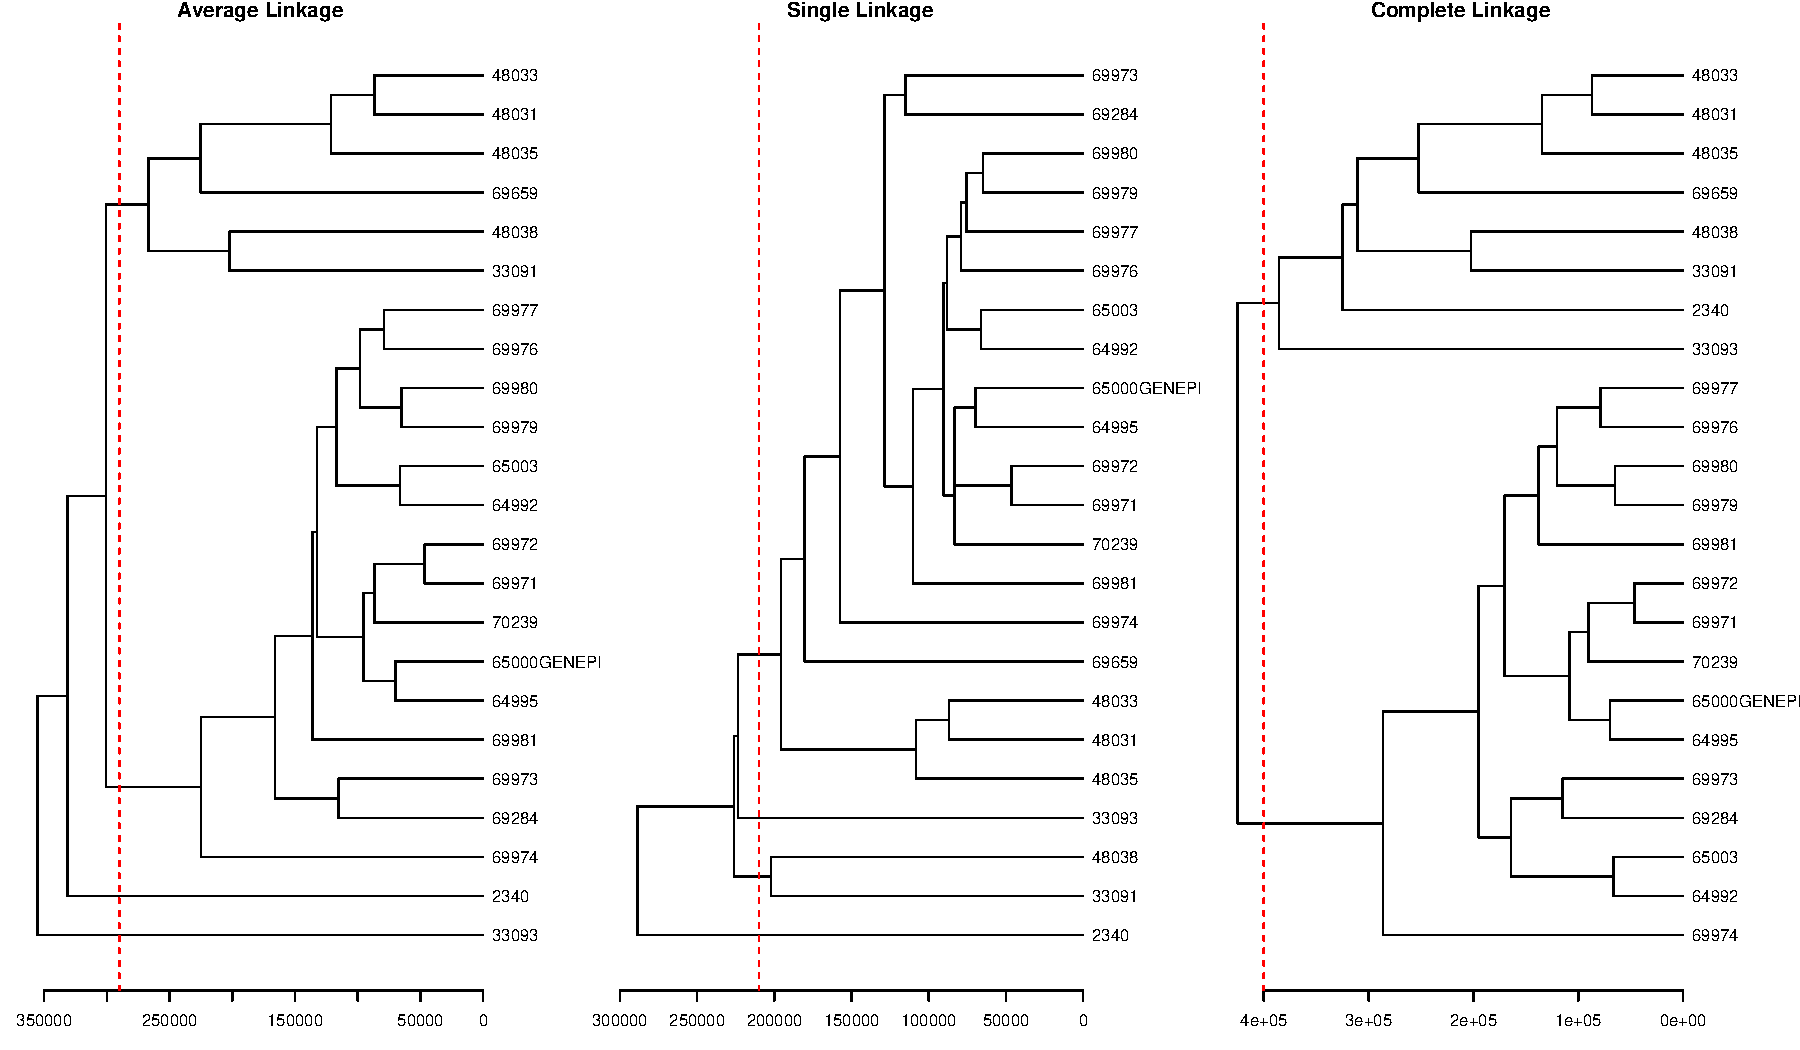
\includegraphics{Osorio_Daniel_HW2-004}
\item Interpret the clusters that you found with respect to the “meta” data for this dataset
\textit{The clusters are mainly driven by the strain type, fuel (10) samples are always clustered together as well as the wine’s (4) samples, depending on the linkage method, the association between strains is recovered differentially.}
\end{enumerate}
\item Carry out K-means clustering, with K = 3. How do the results compare to the hierarchical clustering results you obtained using average linkage? \textit{Main clusters are recovered identically}
\begin{Schunk}
\begin{Sinput}
> avgHclust <- as.dendrogram(avgHclust)
> set.seed(11)
> K <- kmeans(distanceMatrix, centers = 3)
> labelCol <- function(x) {
+   if (is.leaf(x)) {
+     label <- attr(x, "label") 
+     K1 <- names(K$cluster)[K$cluster == 1]
+     K2 <- names(K$cluster)[K$cluster == 2]
+     K3 <- names(K$cluster)[K$cluster == 3]
+     attr(x, "nodePar") <- 
+       list(lab.col=if(label %in% K1){
+       "red"} else {if (label %in% K2){"blue"} else{"green"}})}
+   return(x)
+ }
> avgHclust <- dendrapply(avgHclust, labelCol)
> nodePar <- list(pch = c(NA,NA))
> par(mar=c(3,15,1,15))
> plot(avgHclust, horiz = TRUE, nodePar = nodePar)
\end{Sinput}
\end{Schunk}
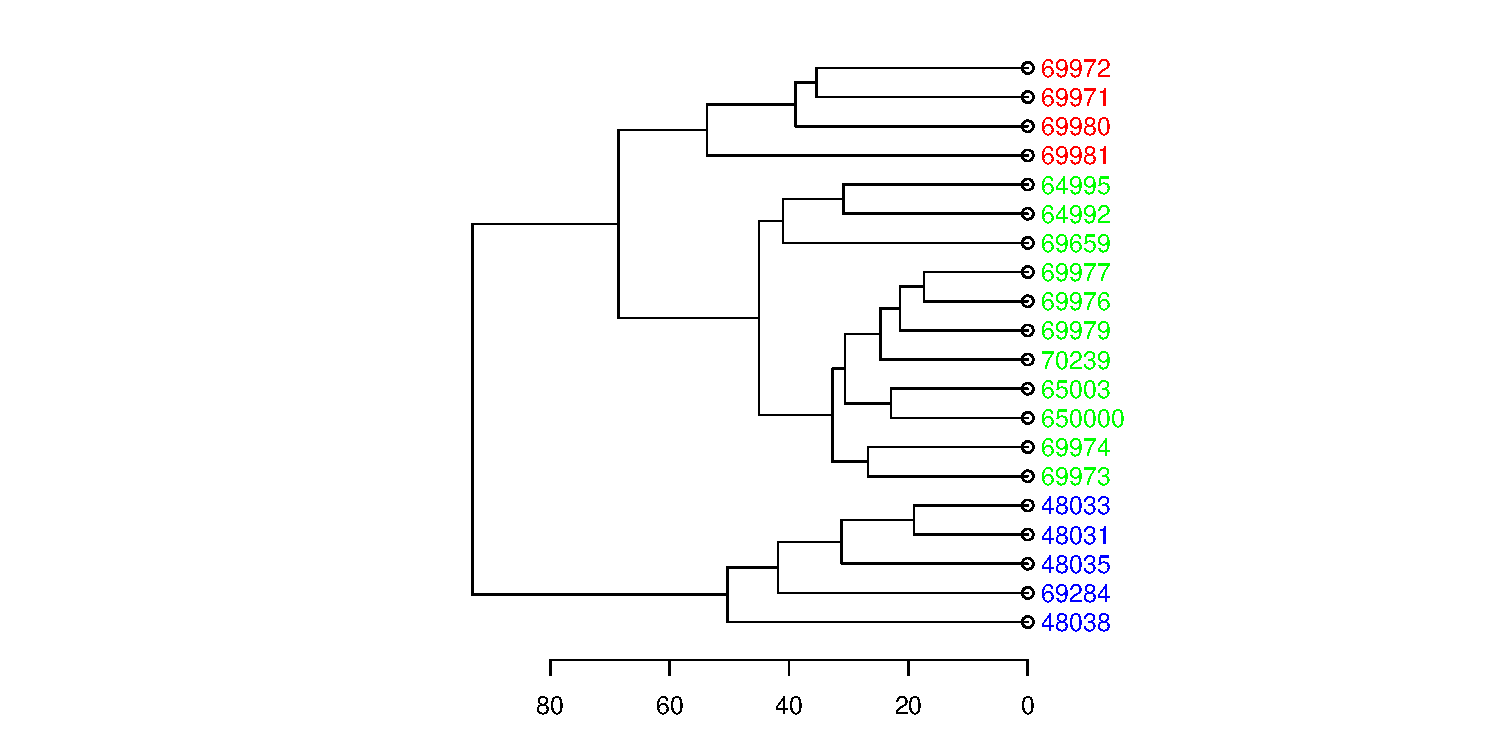
\includegraphics{Osorio_Daniel_HW2-005}
\end{enumerate}
\item The cardiothoracic data, in file `GDS4308.soft', are described here: 
\begin{center}https://www.ncbi.nlm.nih.gov/sites/GDSbrowser?acc=GDS4308\end{center}
Note that the first 97 lines of the data file consist of meta data, so the gene intensities start
on line 98. Note also that the last line of the data file contains a table description and should
not be included with the gene intensities. In what follows, work with the log2-transformed
intensities. Inspect the meta data in “GDS4308.soft” (you can just open it in a text editor)
to figure out what the column names correspond to. Note that these are paired data.
\begin{Schunk}
\begin{Sinput}
> GSE19533 <- read.csv(file = "GDS4308_full.soft", 
+                      sep = "\t", skip = 122, 
+                      comment.char = "!")
> GSE19533 <- log2(GSE19533[,3:12])
\end{Sinput}
\end{Schunk}
\begin{enumerate}
\item Carry out hierarchical clustering of the individuals, using Euclidean distance and complete linkage. Interpret the results.
\begin{Schunk}
\begin{Sinput}
> dGSE19533 <- dist(t(GSE19533))
> hc <- hclust(dGSE19533, method = "complete")
> par(mar=c(3,15,1,15))
> plot(as.dendrogram(hc), horiz = TRUE)
\end{Sinput}
\end{Schunk}
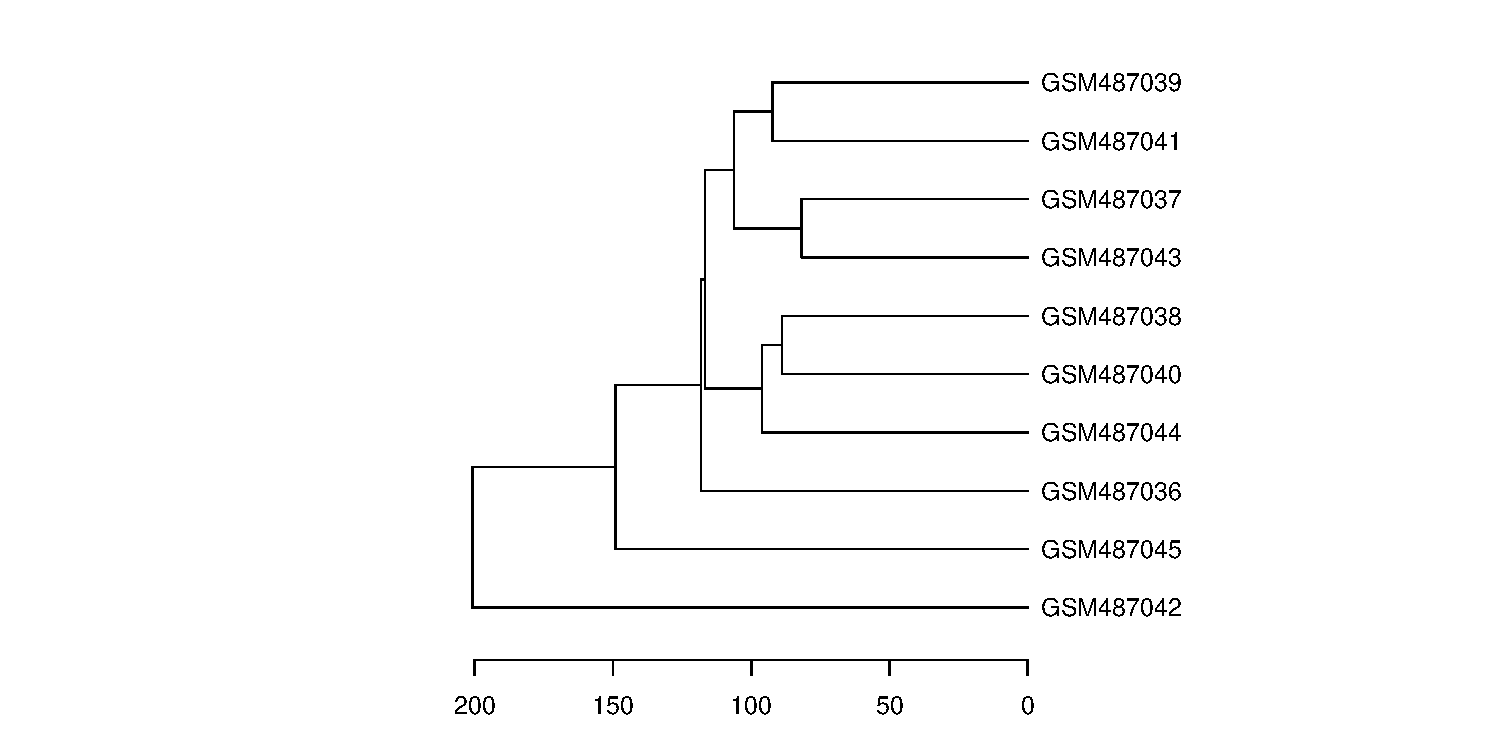
\includegraphics{Osorio_Daniel_HW2-007}
\\\textit{Clusters are driven by the state of the surgery, pre- and post- surgery samples are mainly clustered together.}
\item Carry out a principal component analysis of the intensities, treating individuals (columns)
as variables and features (rows) as replicates. Interpret the results.
\begin{Schunk}
\begin{Sinput}
> cGSE19533 <- t(scale(t(GSE19533)))
> PC <- prcomp(t(cGSE19533))
> barplot(PC$sdev/sum(PC$sdev))
> plot(PC$x[,1:2])
\end{Sinput}
\end{Schunk}
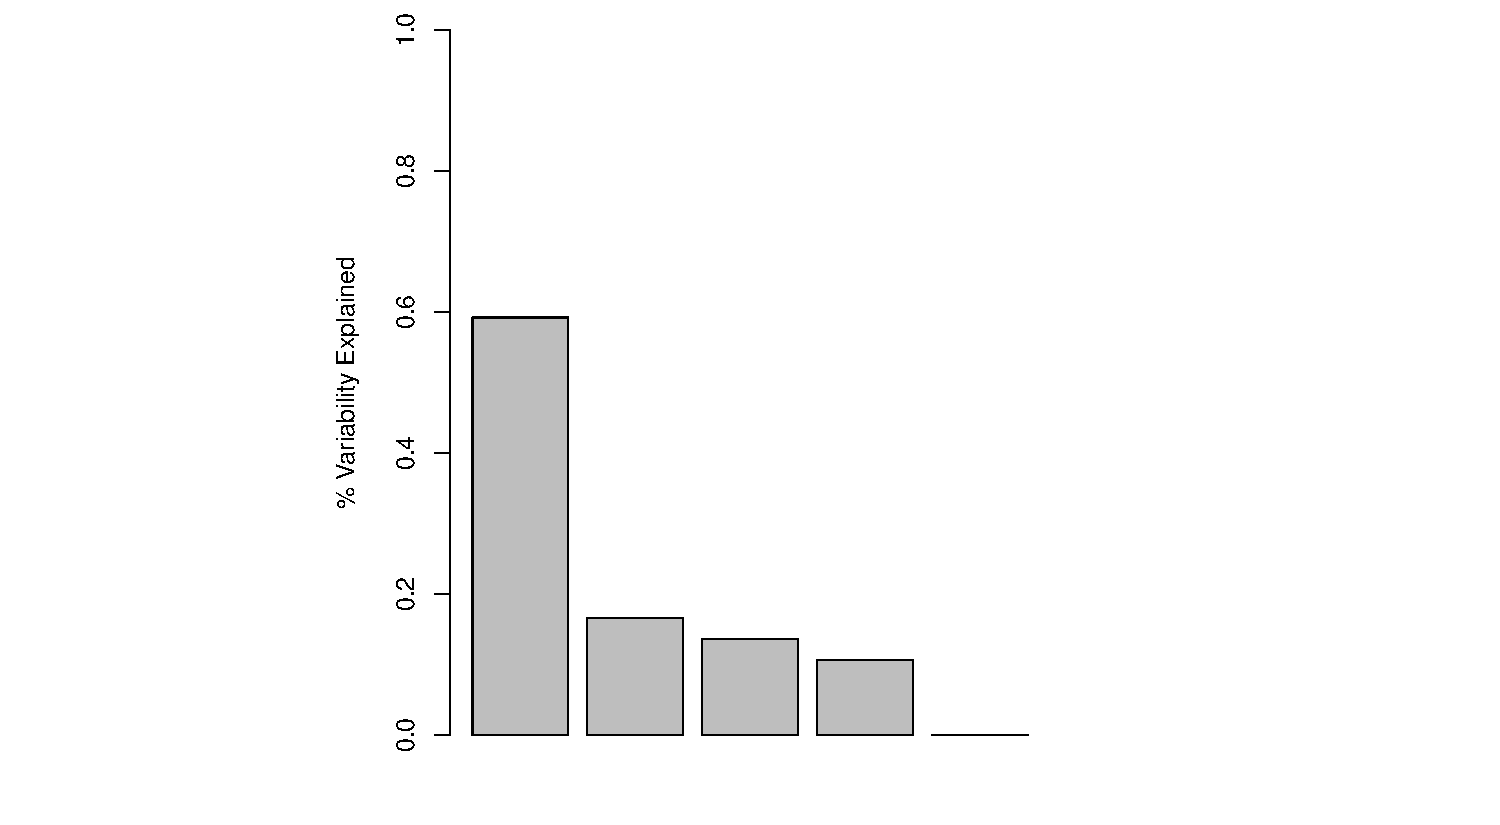
\includegraphics{Osorio_Daniel_HW2-008}
\item Carry out singular value decomposition of the column-centered intensities. Interpret the
results.
\begin{Schunk}
\begin{Sinput}
> SVD <- svd(t(cGSE19533))
\end{Sinput}
\end{Schunk}
\includegraphics{Osorio_Daniel_HW2-009}
\item Compute one-sample t-statistics for each gene to search for features for which the mean
paired difference is not 0. Use the bootstrap to obtain p-values. Use p.adjust to translate
the p-values to FDR estimates (specify argument method = ‘fdr’). How many features
are significant at an estimated FDR of 0.05? I will give tips on R code for this problem
in class and Q\&A.
\begin{Schunk}
\begin{Sinput}
> pre <- paste0("GSM4870",seq(37,45,2))
> pos <- paste0("GSM4870",seq(36,44,2))
> pre <- t(scale(t(GSE19533[,pre]), center = TRUE, scale = TRUE))
> pos <- t(scale(t(GSE19533[,pos]), center = TRUE, scale = TRUE))
> diff <- GSE19533[,pos] - GSE19533[,pre]